%%
%% This is file `mcmthesis-demo.tex',
%% generated with the docstrip utility.
%%
%% The source files were:
%%
%% mcmthesis. dtx  (with options: `demo')
%% !Mode:: "TeX:UTF-8"
%% -----------------------------------
%% This is a generated file.
%% 
%% Copyright (C) 2010 -- 2015 by latexstudio
%%       2014 -- 2019 by Liam Huang
%%       2019 -- present by latexstudio.net
%% 
%% License: The LaTeX Project Public License 1.3c
%% 
%% The Current Maintainer of this work is latexstudio.net.
%% 
\documentclass{mcmthesis}
 %\documentclass[CTeX = true]{mcmthesis}  % 当使用 CTeX 套装时请注释上一行使用该行的设置
\mcmsetup{tstyle=\color{black}\bfseries,%修改题号,队号的颜色和加粗显示,黑色可以修改为 black
        tcn = 2400430, problem = C, %修改队号,参赛题号
        sheet = true, titleinsheet = true, keywordsinsheet = true,%修改sheet显示信息
        titlepage = false, abstract = true}

  %四款字体可以选择
  %\usepackage{times}
  \usepackage{newtxtext,newtxmath} %CTeX 无此字体,可用 txfonts 替代,请使用新版 TeXLive.
  %\usepackage{palatino}
  %\usepackage{txfonts}

\usepackage{indentfirst}  %首行缩进,注释掉,首行就不再缩进。
\usepackage{lipsum}
\usepackage{booktabs}
\usepackage{listings}
\usepackage{color}
\usepackage{enumitem}
\usepackage{amsmath}
\usepackage{algorithm}
\usepackage{algpseudocode}
\usepackage{tikz}
\usepackage{caption}
\usetikzlibrary{positioning, arrows, calc}

% Define custom colors
\definecolor{codegreen}{rgb}{0,0.6,0}
\definecolor{codegray}{rgb}{0.5,0.5,0.5}
\definecolor{codepurple}{rgb}{0.58,0,0.82}
\definecolor{backcolour}{rgb}{0.95,0.95,0.92}

% Custom style for listings
\lstdefinestyle{mystyle}{
    backgroundcolor=\color{backcolour},   
    commentstyle=\color{codegreen},
    keywordstyle=\color{magenta},
    numberstyle=\tiny\color{codegray},
    stringstyle=\color{codepurple},
    basicstyle=\ttfamily\footnotesize,
    breakatwhitespace=false,         
    breaklines=true,                 
    captionpos=b,                    
    keepspaces=true,                 
    numbers=left,                    
    numbersep=5pt,                  
    showspaces=false,                
    showstringspaces=false,
    showtabs=false,                  
    tabsize=2
}

% Set the default style for listings
\lstset{style=mystyle}

\title{Momentum with Counter-Factual Multi-LGBM Chain}
\author{\small \href{https://www.latexstudio.net/}
  {\includegraphics[width=7cm]{mcmthesis-logo}}}
\date{\today}
\begin{document}
\begin{abstract}
\par Our research paper analyzes the influence and characteristics of "momentum" in tennis. To achieve this goal, we have identified features that affect tennis players and used them to train our network. We used a Light Gradient Boosting Machine (LGBM) for supervised learning and predicted the probability of each player scoring at every match moment. This approach helps us evaluate which player performs better at specific times during the game. We also visualize the game's dynamics by plotting the win probability of each point for a player.

We explore the idea of "momentum" in tennis by conducting a series of calculations. This concept is closely related to the effect of each point on the win probability of the entire game, set, or match. To calculate leverage and momentum, we have designed a multi-LGBM chain that substantiates the strong association between momentum and player performance using indicators such as continuous scoring and the weighted sum of win possibilities. Our findings reveal a correlation between momentum and performance, which offers insight for coaches to devise more effective strategies in tennis matches.

We propose the critical factors that determine the flow of a tennis game and their correlations. We aim to improve the advice provided to athletes. We are building on our previous research and choosing additional' multi-probability indices.' It is the weighted sum of predicted win probability in points, games, sets, or matches. We use this to determine the swing of the game and study the relationship between these swings and momentum. The weight here can be perceived as a measure of how farsighted a player is. Our methodology helps us predict and measure the game's fluctuations and identify the most vital indicators.

We tested our models using diverse and representative datasets to make them more reliable. We also evaluate model performance in competitive settings and identify factors to improve future model accuracy. This ensures that our models can be applied with precision in various competitions or tournaments.

In summary, this study provides a detailed analysis of "momentum" in tennis. It utilizes LGBM models and introduces a new "leverage" metric to evaluate momentum's impact on player performance, particularly during critical match moments. The study also identifies the key indicators of match flow and their correlations with momentum. The model's accuracy and applicability in the real world have been tested on diverse datasets, making it a significant achievement in tennis sports analytics and strategic planning.

All the code and figures will be released on \url{https://github.com/BorisGuo9/2024_MCM.git} once the submission of MCM 2024 is closed.

\begin{keywords}
Momentum in tennis, Light Gradient Boosting Machine(LGBM), Counter-Factual analysis, Multi-LGBM chain, Exponentially Weighted Moving Average (EWMA), Markov Chain, Multi-probability, Analytic Hierarchy Process (AHP)
\end{keywords}
\end{abstract}
\maketitle
%% Generate the Table of Contents if it's needed.
\tableofcontents
\newpage
%%

\section{Introduction}
\subsection{Problem Background}
The Wimbledon Championships, founded in 1877, is a prestigious tennis tournament in Wimbledon, England. It's one of the four Grand Slams, usually held in June or July.

Just like any other sporting event, the outcome of Wimbledon is intense and full of unknowns. The situation on the court is ever-changing, and some players can turn the tables and win. These fantastic twists and turns in the game are often caused by the player's "momentum." However, this "momentum" is usually a subjective judgment, defined in sports as the force or intensity gained by a sequence of events or movements, so it is often difficult to measure this phenomenon, and it is not always easy to identify how events in a match can create or change the momentum.

\subsection{Restatement of the Problem}
The 2024 MCM Problem C is centered around the concept of "momentum" in tennis matches. The requirement is that our model should not only capture the match flow for scoring performance but also go on to predict the momentum. This model should include visualizations of match flow and consider the higher win probability of points for the serving player.

In addition, the problem requires an assessment of the claim by a tennis coach that swings in play and runs of success are random rather than due to momentum. To achieve this, the model needs to identify indicators predicting swings in the match's flow, analyze data from past matches, and advise players on preparing for new matches against different opponents.

The challenge extends beyond just developing the model. It also involves testing the model on other matches to determine its generalizability across various matches, tournaments, court surfaces, and other sports like table tennis. Finally, the problem requires a report with a maximum length of 25 pages, summarizing findings and offering a memo for coaches on momentum and match flow response strategies.

\subsection{Preliminary}
\subsubsection{Preliminary of LGBM}
In our paper, we implement LightGBM (Light Gradient Boosting Machine), a framework based on the Gradient Boosting Decision Tree (GBDT) algorithm. GBDT, a well-established model in machine learning, builds the optimal model through iterative training of weak classifiers, namely decision trees. This approach offers benefits like practical training and resistance to overfitting. GBDT is not only prevalent in the industry for applications like multi-classification, click-through rate prediction, and search ranking but also a powerful tool in data mining competitions. 

LightGBM, enhancing the GBDT algorithm, supports high-efficiency parallel training. This results in faster training speeds, reduced memory usage, improved accuracy, and the ability to handle large-scale data efficiently, making it a robust solution in various data processing scenarios.

\subsubsection{Other Literatures Overview}
We read multiple papers about momentum, machine learning analysis, and counter-factual analysis in tennis games.

Literature \cite{1} introduces a counter-factual approach in women's tennis, using metrics like "leverage," "clutch," and "momentum" to identify key moments in matches automatically. This method goes beyond the traditional focus on breakpoints, predicting the impact of each point on the match outcome, including comeback potential. It can foresee crucial moments and link player behaviors to their tendencies in pivotal situations.

Literature \cite{4} provides the perspective from machine learning analysis of tennis games, and other papers include probability-based models, stochastic modeling of individual points in a match \cite{8}, combining player statistics \cite{7}, and  algorithms like LightGBM for analyzing and predicting match outcomes \cite{11}. Studies range from specific analysis of single matches to assessing player performances over a season, showcasing the extensive application of data science in sports \cite{5}.

\section{Assumptions and Parameters}
\subsection{Assumptions}
\begin{enumerate}
  \item \textbf{Match Dynamics}: Assume the dynamics of a tennis match, such as scoring and games, can be accurately modeled using quantitative methods.
  \item \textbf{Data Accuracy}: Assume the provided data, including match details and player statistics, is reliable and sufficient for the model.
  \item \textbf{Predictive Modeling}: Assume it is possible to create a predictive model for match outcomes based on historical data and current match conditions.
  \item \textbf{Performance Variability}: Recognize inconsistency in how players perform in various matches, on different surfaces, and over time.
\end{enumerate}

\begin{table}[ht]
\centering
\begin{tabular}{p{0.2\linewidth}p{0.3\linewidth}p{0.4\linewidth}}
   \toprule
   \textbf{Parameter} & \textbf{Description} & \textbf{Details} \\
   \midrule
   $P_\textit{xxWin}$ & win probability & \emph{xx} can be point, game,set and match \\
   $P_\textit{mul}$ & multi-probability & weighted sum of 4 win probabilities \\
   $k$ & point number & player scored k\textsuperscript{th} point \\
   $x_k$ & leverage values & value of leverage of k\textsuperscript{th} point \\
   $\alpha$ & smoothing factor & smoothing factor in  EWMA \\
   $r$ & pearson coefficient & strength of the linear relationship \\
   $X_i$,$Y_i$& variables values & observed values of X and Y \\
   $\bar{X}$, $\bar{Y}$& variables means & sample means of X and Y \\   
   \bottomrule
\end{tabular}
\caption{Model Parameters Definition}
\label{tab:parameters}
\end{table}

\subsection{Parameters}
The table \ref{tab:parameters} shows the parameters that appear in this article.

\section{Data Preparation}
\subsection{Data Collection}
The \emph{Wimbledon\_featured\_matches.csv} file contains detailed information about Wimbledon 2023 tennis matches. It includes player identification and specific tennis metrics like scores, service details, and point outcomes. The dataset captures the dynamics of each point within matches, enabling an in-depth analysis of player performance and match strategy.\AIcite{AI2}

We collected tennis and badminton match datasets from the US Open Tennis and BWF World Tour tournaments to improve generalization. The \emph{2023-usopen-points.csv} file and \emph{badminton\_data.csv} file also contains match progression details, showing the diversity of data objects our model applies to.

\subsection{Data Cleaning}
We notice missing values in the columns speed\_mph and return\_depth in our dataset. To handle this issue, we apply a data-cleaning strategy. For columns like speed\_mph and return\_depth, we fill the missing values with the mean of the respective columns. This approach provides a reasonable approximation of the missing data. We also identify outlier values in the columns p1\_score and p2\_score. These outliers are values that fell outside the typical scoring range in the dataset. To deal with this, we convert the scores into points within an acceptable range. This process helps to maintain the dataset's integrity.\AIcite{AI1}

In addition to this, we separate the match\_id field into two separate fields: round\_no and match\_no. This separation allows us to analyze the matches more precisely, facilitating better insights into the data's patterns and trends. Furthermore, we transform specific categorical values into binary values, such as CTL, NCTL, D, and ND, and we convert the \emph{Hour-Minute-Second} format to seconds. This transformation simplified the dataset and made it more suitable for the analytical models we plan to use later in our study.

\section{Task I: Performance Evaluation by LGBM}
\subsection{Task Review and Approach}
For this task, we need to create a model that can track the match flow as points are scored. This model will be applied to one or more matches and should be able to determine which player is performing better at any given moment. Additionally, We provide a visual representation of the match flow based on our model.

To achieve this requirement, we use LGBM, which is a machine learning method. The main idea is to use weak classifiers (decision trees) to train to get the optimal model iteratively. We clean the raw data and then segment it to get features for feature engineering. Then, cut the training set and the validation set for training the model and testing the network. The input to this model is the features we extract from the original dataset and the score situation, and the output is the probability that the player will score the point in the current situation.

\subsection{Implementation of LGBM}
\subsubsection{Data Segmentation for LGBM}
LGBM requires multiple features to form classifiers to build decision tree models. So, we implement the segmentation on original data for feature engineering.

The extracted features are as follows:
\begin{itemize} \setlength\itemsep{0em}
    \item $x_1$: Number of games lead in the current set.
    \item $x_2$: Scores lead in the current game.
    \item $x_3$: Binary indicator of whether player 1 is the Server (1) or not (0).
    \item $x_4$: Number of sets lead in the match.
    \item $x_5$ to $x_8$: Binary indicators for events in the current game, such as ace, winner, double fault, and unforced error by player 1.
    \item $x_9$: Ratio of net points won to total net points played by player 1.
    \item $x_{10}$: Ratio of break points won to total break points played by player 1 in the set.
    \item $x_{11}$: Total distance run by player 1 in the match up to the current point.
    \item $x_{12}$: Total distance run by player 1 in the last three points.
    \item $x_{13}$: Distance run by player 1 in the last point.
    \item $x_{14}$: Ball speed.
    \item $x_{15}$: Number of hits in the rally.
    \item $x_{16}$: Depth of serve or return, depending on whether player 1 is serving or returning.
\end{itemize}
In a match, every point is closely examined, and features $x_1$ to $x_{16}$ are calculated based on the analysis. Additionally, each point is tagged with the name of the player who won it, whether it is player 1 or player 2. It's worth noting that the \emph{Server}, corresponding to $x_3$, is included in the features because the server has a higher win probability.

\subsubsection{Training and Verification of LGBM}
Efficient handling of high-dimensional features is a crucial aspect of training an LGBM model for optimal performance. The sparsity characteristic of high-dimensional data, with many feature values zero, allows us to bundle certain features that are mutually exclusive without any loss of information. Our approach introduces the concept of a conflict ratio to quantify the degree of overlap between features that are not entirely mutually exclusive. By tolerating a small conflict ratio, we can reduce the number of feature bundles and enhance computational efficiency, allowing for dimensionality reduction without significant loss of information.

It is important to note that even a slight contamination in the feature space (due to overlapping features) can impact the model's accuracy. However, if this contamination is kept minimal, it can provide an optimal trade-off between accuracy and computational efficiency. To implement this approach in LGBM, we recommend the following steps:
\begin{enumerate}
    \item Construct a weighted undirected graph where vertices are features and edges have weights that are related to the conflict between two features;
    \item Sort the nodes in descending order according to their degree; the greater the degree, the greater the conflict with other features;
    \item Iterate each feature and assign it to an existing feature package or create a new one such that the overall conflict is minimized.
\end{enumerate}
The pseudo-code for the feature bundling in the LGBM algorithm is shown below:
\begin{algorithm}
\caption{Feature Bundling in LGBM}
\label{bundling}
\begin{algorithmic}[1]
\Require $F$: features, $K$: max conflict count
\State Construct graph $G$
\State $searchOrder \gets G.sortByDegree()$
\State $bundles \gets \{\}$, $bundlesConflict \gets \{\}$
\For{$i$ in $searchOrder$}
    \State $needNew \gets \text{True}$
    \For{$j \gets 1$ to $\text{len}(bundles)$}
        \State $cnt \gets \text{ConflictCnt}(bundles[j], F[i])$
        \If{$cnt + bundlesConflict[i] \leq K$}
            \State $bundles[j].add(F[i])$, $needNew \gets \text{False}$
            \State \textbf{break}
        \EndIf
    \EndFor
    \If{$needNew$}
        \State Add $F[i]$ as a new bundle to $bundles$
    \EndIf
\EndFor
\Ensure $bundles$
\end{algorithmic}
\end{algorithm}

After bundling the feature, the dataset is divided into training and testing datasets using an 80-20 split ratio. After that, we set certain parameters for the LGBM model, such as the objective being set as 'binary,' the metric being set as 'auc,' and other parameters like num\_leaves, learning\_rate, etc. The model is trained with 400 iterations and early stopping after 50 rounds. The predictions are then made on the test set. These predictions are then converted to binary format (1 or 0) based on a threshold of 0.5. The model's accuracy and classification report are generated and printed. Finally, we apply the model to a new dataset ('standard predict performance.csv') to predict performance scores. The predictions are saved to \emph{Predicted Performance.csv}.

\subsection{Results and Analysis}

Fig.\ref{fig:score} shows the Performance score, which presents the win probability at a given point of a player and whether they are performing better at that point in the match. We use the LOWESS method from the statsmodel package in Python to smooth the trend line and understand performance patterns for coaching strategies, player development, and match play tactics. The smoothed curve shows how well a player has performed over a certain period.

The classification report in Table \ref{tab:classification_report} shows a model with good predictive performance, balanced precision, recall, and F1-score. It has a slight advantage in detecting instances of a split dataset and an overall accuracy of 0.81, which means that it correctly predicts the class 81\% of the time. 

\begin{figure}[ht]
    \centering
    % First Row
    \begin{minipage}{0.4\textwidth}
        \centering
        \includegraphics[width=\textwidth]{figures/conf_matrix.png} % Confusion matrix now in the first position
        \caption{Confusion matrix}
        \label{fig:conf}
    \end{minipage}\hfill
    \begin{minipage}{0.6\textwidth}
        \centering
        \captionof{table}{Classification Report}
        \label{tab:classification_report}
        \begin{tabular}{lcccc}
        \toprule
        Class & Precision & Recall & F1-score & Support \\
        \midrule
        0 & 0.81 & 0.79 & 0.80 & 629 \\
        1 & 0.81 & 0.83 & 0.82 & 678 \\
        \midrule
        \textbf{Accuracy} & & & \textbf{0.81} & \textbf{1307} \\
        \textbf{Macro Avg} & \textbf{0.81} & \textbf{0.81} & \textbf{0.81} & \textbf{1307} \\
        \textbf{Weighted Avg} & \textbf{0.81} & \textbf{0.81} & \textbf{0.81} & \textbf{1307} \\
        \bottomrule
        \end{tabular}
    \end{minipage}
    
    % Second Row
    \begin{minipage}{0.55\textwidth}
        \centering
        \includegraphics[width=\textwidth]{figures/smooth_curve.png} % Performance score now in the third position
        \caption{Performance score}
        \label{fig:score}
    \end{minipage}\hfill
    \begin{minipage}{0.45\textwidth}
        \centering
        \includegraphics[width=\textwidth]{figures/ROC_Curve.png} % ROC Curve remains in the fourth position
        \caption{Receiver operating characteristic curve}
        \label{fig:ROC}
    \end{minipage}
\end{figure}

Fig. \ref{fig:conf} and Fig. \ref{fig:ROC} indicate the Confusion matrix and receiver operating characteristic (ROC) curve separately. A confusion matrix evaluates classification model performance, comparing actual and predicted labels. The ROC curve shows binary classifier accuracy, with an AUC closer to 1 indicating higher accuracy. In this case, AUC is 0.933 a high level of accuracy.

This prediction is based on Wimbledon 2023 round 7 match 1, which has the match id of \emph{20223-wimbledon-1701}. It is the showcase of player \emph{Carlos Alcaraz}. This performance score can benefit our evaluation of each player in each match.

In summary, we divided the dataset into two categories: one for training and the other for validation. The decision trees we developed from the training data yielded remarkable accuracy levels, ranging between 80\% to 90\% when tested against the validation sets. This high accuracy demonstrates the validity of our model in capturing the dynamic flow of play characteristic of the individual athlete's game and reflecting the player's performance. Such results strengthen the robustness of our predictive framework, indicating its potential to accurately gauge match outcomes based on the players' performance metrics.

\section{Task II: Leverage and Momentum with Multi-LGBM chain}
\subsection{Task Review and Our Approach}
Our task is assessing the claim made by a tennis coach that swings in play and runs of success by one player are random and that "momentum" is merely a suspicious concept. To quantify the subjective notion of momentum in tennis, we introduce the concept of leverage. We have developed a multi-LGBM chain based on LGBM, which enables us to perform counter-factual analysis. This approach has proven to be effective in quantifying momentum, which has shown a strong correlation with player performance.

To address the skepticism surrounding the concept of momentum in tennis, it is crucial to establish a clear definition of what momentum is. We begin by defining a metric to evaluate the importance of each point, referred to as leverage. Using leverage, we illustrate the definition of momentum and demonstrate its importance in the match flow.

\subsection{Introduction of Leverage and Momentum}
\subsubsection{Definition of Multi-probability and Leverage}
\label{leverage}
We define multi-probability as the weighted sum of each win probability. It is a key concept that we introduce to quantify the influence of points for the win probability. It is a  win probability measurement based on the Analytic Hierarchy Process(AHP)  with four kinds of probabilities from point, game, set, and match, respectively. The detailed discussion can be found in section \ref{multi-probability}.

We define leverage as measuring how the magnitude of multi-probability changes as a result of either winning or losing the point. Leverage is a concept to measure the importance of every point based on the counter-factual analysis, which can be used to measure the impact of every single point on the outcome of a game, a set, or even a match by framing it as a “what-if” question. We conduct two predictions - the first based on the original outcome and the second on the reverse outcome – and then we compare the difference in prediction output.\cite{1}

In this task, we implement a counter-factual analysis by constructing two scenarios: the real world, which corresponds to the actual dataset, and a hypothetical world, where we reverse the 'point-victor' attribute and then use this modified point scoring data to recalculate the new probabilities of games, sets, and matches. This approach allows us to analyze how outcomes would differ under alternate point-winning scenarios.

\subsubsection{Definition of Momentum}
Built on the defined concept of leverage, momentum is articulated as \textit{“an Exponentially Weighted Moving Average (EWMA) of the leverage accrued by a player at a particular point.”}. The equation to calculate the momentum is as follows.
\begin{equation} \label{eq:momentum}
Momentum = \frac{x_k + (1 - \alpha)x_{k-1} + (1 - \alpha)^2 x_{k-2} + \cdots + (1 - \alpha)^k x_0}{1 + (1 - \alpha) + (1 - \alpha)^2 + \cdots + (1 - \alpha)^k}
\end{equation}
Where $[x_0, x_1, \ldots, x_k]$ are the gained leverages of the last $k$ points with smoothing factor $\alpha$ and $Momentum$ is the momentum at point $k$.

To gain a deeper understanding of the role of momentum in tennis, we should incorporate the idea of Markov chains into its description. Markov chains emphasize that each state of a process is related to the previous state, which is closely linked to the concept of momentum. Momentum takes into account a player's successive performances in a match.

Based on this, the formula for momentum is defined as an exponentially weighted moving average (EWMA) of a player's successive scores in a tennis match. By applying a smoothing factor, denoted by $\alpha$, which assigns more weight to recent scores, the formula captures the essence of momentum. The method produces a dynamically weighted average that reflects a player's changing dominance throughout the game. This approach provides a real-time analysis of momentum fluctuation and a comprehensive understanding of a player's performance flow over time.

It's important to highlight the distinct differences between momentum and leverage in terms of their definition and application. Leverage is non-historical and considers the advantage that a player may gain in a given playing situation, while momentum is historical and related to past performance.

We have developed a model that calculates the win probability of a game, set, and match by analyzing the impact of each point. The model is built using LGBM as the framework in Figure \ref{fig: model} and uses a sequential approach that integrates point-by-point effects to provide a comprehensive win probability of match assessment.

\subsection{Multi-LGBM Chain}
\subsubsection{Indicators}
As impact factors for the win probability model, we divide determinants into three categories: Technical, Psychological, and Physiological. Each category is marked by specific variables, ranging from $x_1$ to $x_{16}$.

Technical Factors refer to personal choices made by the player, such as serving status ($x_3$), aces ($x_5$), winners ($x_6$), double faults ($x_7$), unforced errors ($x_8$), and the ratio of net points won ($x_9$).

Psychological Factors may affect the player's mindset. This is observable through the proportion of break points won ($x_{10}$), the number of sets a player is leading by ($x_1$), the score advantage in the current game ($x_2$), and the number of set leading in the match($x_4$).

Physiological Factors encompass physical metrics such as total distance run in the match ($x_{11}$), in the last three points ($x_{12}$), and in the previous point ($x_{13}$). Additionally, it includes ball speed ($x_{14}$), rally count ($x_{15}$), and the depth of serves or returns ($x_{16}$), which reflect the player's endurance and physical exertion.

Our LGBM model meticulously processes these elements to compute win probabilities from the point level to the overall match outcome.

\subsubsection{Model Structure}

In Figure \ref{fig: model}, you can see that the model has a chain-like structure that calculates the probabilities of winning at different stages in a tennis match. It takes into account critical factors such as Technical, Physiological, and Psychological. It begins with the PointWinner Model, which estimates the win probability of each point based on these factors. This output is then used as input for the GameWinner Model, and so on, through the SetWinner and MatchWinner Models. Each layer builds upon the previous one, resulting in a refined win probability. This sequence effectively captures the various influences and interconnected impacts on a player's performance.

The approach offers a comprehensive and dynamic assessment of match progression. It captures the interplay of various determinants of a player's performance. It enables a granular understanding of how different factors influence the game at different levels, from individual points to the entire match.

\begin{figure}[ht]
    \centering
    \begin{minipage}{\textwidth}
        \centering
        \includegraphics[width=\textwidth]{figures/flow.pdf} 
        \caption{The structure of momentum model}
        \label{fig: model}
    \end{minipage}\hfill
\end{figure}

\subsubsection{Counter-Factual Analysis Based on Multi-LGBM Chain}
Here, we mean "What if the player lost the point which he or she could have won" or "What if the player won the point which he or she could have lost". This what-if problem constructs a hypothetical world that reverses the point victor, causing a probable change in the victor of the game, set, or even match. Based on the counter-factual analysis, we are able to obtain a total of 8 winning probabilities, which are 2 pairs of point, game, set, and match win probability, comprising four from the original data set and another four from data where the point outcomes are reversed.

Our Multi-LGBM model allows us to calculate four unique win probabilities for a player at different stages of point, game, set, and match each time a point is scored. You can refer to Fig. \ref{fig:momentum} for a visual representation of this process. 

\begin{figure}[ht]
    \centering
    \begin{minipage}{\textwidth}
        \centering
        \includegraphics[width=0.9\textwidth]{figures/momentum.pdf} 
        \caption{The process of counter-factual}
        \label{fig:momentum}
    \end{minipage}\hfill
\end{figure}

\subsection{Experiment}
\subsubsection{Calculate on Leverage}
Based on the prior work in section \ref{leverage} and the outcome of the counter-factual analysis, we are able to calculate the leverage. We utilize AHP to process the probabilities from the same source of data in order to obtain an index that is able to represent the overall influence of win probability for a single point, which we named multi-probability in the coming section \ref{multi-probability}.
The calculation of leverage is shown in the equation below:
\begin{equation} \label{eq:leverage}
Leverage = P_\textit{mul}( \textbf{Real}) - P_\textit{mul}( \textbf{Hypo})
\end{equation}
Where $P_\textit{mul}( \textbf{Real})$ stands for the multi-probability comes from the original dataset, and the $P_\textit{mul}( \textbf{Hypo})$ stands for the multi-probability comes from the reverse dataset. Utilizing this equation, we can obtain the leverage for every point of one player.

\subsubsection{Calculate on Momentum}
After calculating the leverage, we compile a list of leverage values for each data point. Subsequently, we initiate the calculation of momentum using the equation in \ref{eq:momentum}, thereby determining the momentum for each point.

The pseudo-code for the conducting from wins to multi-probability to leverage to momentum is shown below:
\begin{algorithm}
\caption{Conducting to Momentum}
    \begin{algorithmic}[1]
        \Procedure{Wins -> Multi-probability}{$Point\_victor, F: Features$}
        \State Use LGBM to calculate $P_\textit{PointWin}$, $P_\textit{GameWin}$, $P_\textit{SetWin}$, $P_\textit{MatchWin}$
        \State Use AHP to decide the weight $\lambda_1, \lambda_2, \lambda_3, \lambda_4$ for $P_\textit{PointWin}$, $P_\textit{GameWin}$, $P_\textit{SetWin}$, $P_\textit{MatchWin}$
        \State Calculate Multi-probability by $P_\textit{mul}$ = $\lambda_1 \times P_\textit{PointWin} + \lambda_2 \times P_\textit{GameWin} + \lambda_3 \times P_\textit{SetWin} + \lambda_4 \times P_\textit{MatchWin}$
        \EndProcedure
        \Procedure{Multi-probability -> Leverage}{$Previous Procedure$}
        \State Illustrate real world and hypothetical world and simulate to MatchWin
        \State Calculate each world using $Previous Procedure$ to get $P_\textit{mul}( \textbf{Real})$ and $P_\textit{mul}( \textbf{Hypo})$
        \State Calculate $Leverage$ = $P_\textit{mul}( \textbf{Real})$ - $P_\textit{mul}( \textbf{Hypo})$
        \EndProcedure
        \Procedure{Leverage -> Momentum}{$Leverage, \alpha$}
        \State Calculate $x_k$ as the leverage of k\textsuperscript{th} point
        \State Calculate $Momentum = \frac{x_k + (1 - \alpha)x_{k-1} + (1 - \alpha)^2 x_{k-2} + \cdots + (1 - \alpha)^k x_0}{1 + (1 - \alpha) + (1 - \alpha)^2 + \cdots + (1 - \alpha)^k}$
        \EndProcedure
        \State Plot $Momentum$
    \end{algorithmic}
\end{algorithm}

\subsection{Correlation between Swings and Momentum}
We evaluate the "swings" in the game by the features in a player's data, and these features are win probability of points, win probability of games, win probability of matches, and consecutive victories, which means a player continuously wins points. 

Utilizing Pearson Correlation Eq. \ref{eq:Pearson}, We obtain the correlation coefficient between momentum and probabilities and consecutive victories, visualizing them into a heatmap in Fig. \ref{fig:correlation} for analysis.

\begin{equation} 
\label{eq:Pearson}
r = \frac{\sum (X_i - \bar{X})(Y_i - \bar{Y})}{\sqrt{\sum (X_i - \bar{X})^2 \sum (Y_i - \bar{Y})^2}}
\end{equation}
\subsection{Result and Analysis}
\subsubsection{Prediction of Momentum}

\begin{figure}[ht]
    \centering
    \begin{minipage}{\textwidth}
        \centering
        \includegraphics[width=1\textwidth]{figures/Momentum_Predication.pdf} 
        \caption{Predicted momentum of Match \#1701}
        \label{fig:Momentum_Predication}
    \end{minipage}
\end{figure}
The momentum we define has a strong real-world correlation, enabling us to analyze, to a considerable extent, the impact of momentum on the progression of the match. To conduct further analysis, we utilize our model to predict the momentum of the 2023 Wimbledon Gentlemen’s Final, a representative match in the world of tennis. Fig. \ref{fig:Momentum_Predication} shows the momentum during the entire match. 

At the beginning of the match, Novak Djokovic delivered an excellent performance, winning five consecutive games. As a result, with high spirits and overwhelming momentum, he dominated the opponent. Even though the opponent caught up in one game towards the end, it was too late to turn the tide. In the second set, Carlos Alcaraz bounced back from the setback in the first set, going head-to-head with Djokovic. The atmosphere was tense, and from the momentum chart, you could observe continuous fluctuations. However, overall, his momentum remained greater than that of his opponent. In the end, he withstood the pressure, won the tiebreaker, and secured victory in this set. 

During the third set, Alcaraz took control of the entire set. His momentum completely overshadowed the opponent, and he easily got the victory. In the fourth set, he couldn't maintain the momentum from the previous set. He failed to create a gap against Djokovic in the early stages and consecutively lost four games during the set. With a declining momentum, he ultimately lost the set 3 $:$ 6. In the last set, he gained a lead with a high momentum. However, Djokovic made a comeback, winning several games. As the match progressed, he got closer to victory with the higher momentum. He withstood Djokovic's pursuit and ultimately won the entire match.

The analysis reveals that momentum indeed exists and exerts an influence on the course of the match, which shouldn't be ignored in tennis matches. 

\begin{figure}[ht]
    \centering
    \begin{minipage}{\textwidth}
        \centering
        \includegraphics[width=0.6\textwidth]{figures/correlation.png} 
        \caption{The correlation heatmap between momentum and features}
        \label{fig:correlation}
    \end{minipage}\hfill
\end{figure}

\subsubsection{Correlations Analysis of Momentum}   

From the heatmap Fig. \ref{fig:correlation}, we can observe obvious correlations between momentum and the features we use to measure the swing of the game. Particularly, the correlation between consecutive victories and momentum is 0.81, which illustrates a strong correlation between them, and the win probability of a match also shows a relatively strong correlation with momentum, which is far higher than the point, game, and set probabilities. This outcome strongly proves that momentum plays an important role in the prediction of the overall performance rather than a short-sighted index only predicting the performance in the small unit of a match.

All of the outcomes can demonstrate that the momentum we define has a strong correlation with the swing in the game and runs of success, powerfully responding to the suspicion about the impact of momentum.

\section{TASK III: Decisive Indicators of the Flow}
\subsection{Task Review}
This task involves developing a predictive model using tennis match data to identify indicators that signal a change in the match's flow, potentially altering the balance of play between players. It encompasses two sub-tasks:

Model Development: Utilize the provided data from at least one match to create a model that can predict swings in the match. This involves analyzing which factors are most closely related to these swings.

Strategic Advice: Based on the model's insights into momentum swings from past matches, formulate strategies or recommendations for a player entering a new match against a different opponent, considering the historical momentum patterns observed.

\subsection{Multi-probability}\label{multi-probability}
\subsubsection{Introduction of Multi-probability and Match flow}
Multi-probability combines win probabilities from point, game, set, and match. It is the weighted sum of probability when a point, game, set, or match wins. The specific process is shown below: 

Initially, employ the LGBM to compute the $P_\textit{PointWin}$, $P_\textit{GameWin}$, $P_\textit{SetWin}$, $P_\textit{MatchWin}$. Subsequently, utilize the  Analytic Hierarchy Process (AHP), which is mentioned in section \ref{ahp}, to ascertain the corresponding weights $\lambda_1, \lambda_2, \lambda_3, \lambda_4$ for these four values. Eq. \ref{Eq: mul} indicates the calculation of multi-probability through a linear weighting approach.

\begin{equation}
\label{Eq: mul}
    P_\textit{mul} = \lambda_1 \times P_\textit{PointWin} + \lambda_2 \times P_\textit{GameWin} + \lambda_3 \times P_\textit{SetWin} + \lambda_4 \times P_\textit{MatchWin}
\end{equation}

By considering these four probabilities, it reflects the ebb and flow of a match and indicates which player holds an advantage. To calculate the weights of these combinations, we're thinking of using the AHP. This method considers the importance of four probabilities, helping us evaluate and assign appropriate weights to them in the overall assessment of multi-probability. We utilize multi-probability to signify changes in the match flow, serving as an assessment of the evolving situations during the match.
\begin{figure}[ht]
    \centering
    \begin{minipage}{0.8\textwidth}
        \centering
        \includegraphics[width=\textwidth]{figures/match_flow.pdf} % first image
        \caption{Match flow predicted by Multi-probability}
        \label{fig:match_flow}
    \end{minipage}\hfill
\end{figure}

\subsubsection{Implementation of AHP}
\label{ahp}
To calculate the weights of the probabilities, it's crucial to initially assess their importance. Therefore, the win probability of the match is deemed vital, followed by the win probability of the set in the second position. Subsequently, the game is considered, with the least importance assigned to the point, contributing relatively minimally to the overall match flow. Thus, the order of importance is match, set, game, and point. 

We quantify their relative importance and construct a Judgment Matrix of AHP. The matrix is as follows:
\[
\begin{bmatrix}
1 & a_{12} & \cdots & a_{1n} \\
\frac{1}{a_{12}} & 1 & \cdots & a_{2n} \\
\vdots & \vdots & \ddots & \vdots \\
\frac{1}{a_{1n}} & \frac{1}{a_{2n}} & \cdots & 1
\end{bmatrix}
\quad
=
\quad
\begin{bmatrix}
1 & 1.33 & 1.67 & 2 \\
0.75 & 1 & 1.33 & 1.67 \\
0.6 & 0.75 & 1 & 1.33 \\
0.5 & 0.6 & 0.75 & 1
\end{bmatrix}
\]
The corresponding weights of the matrix are $[0.349, 0.273, 0.212, 0.166]$. The relations between the goal, criteria, and options are indicated in Fig. \ref{fig:my_map}.
\begin{figure}[ht]
\centering
\resizebox{0.7\textwidth}{!}{

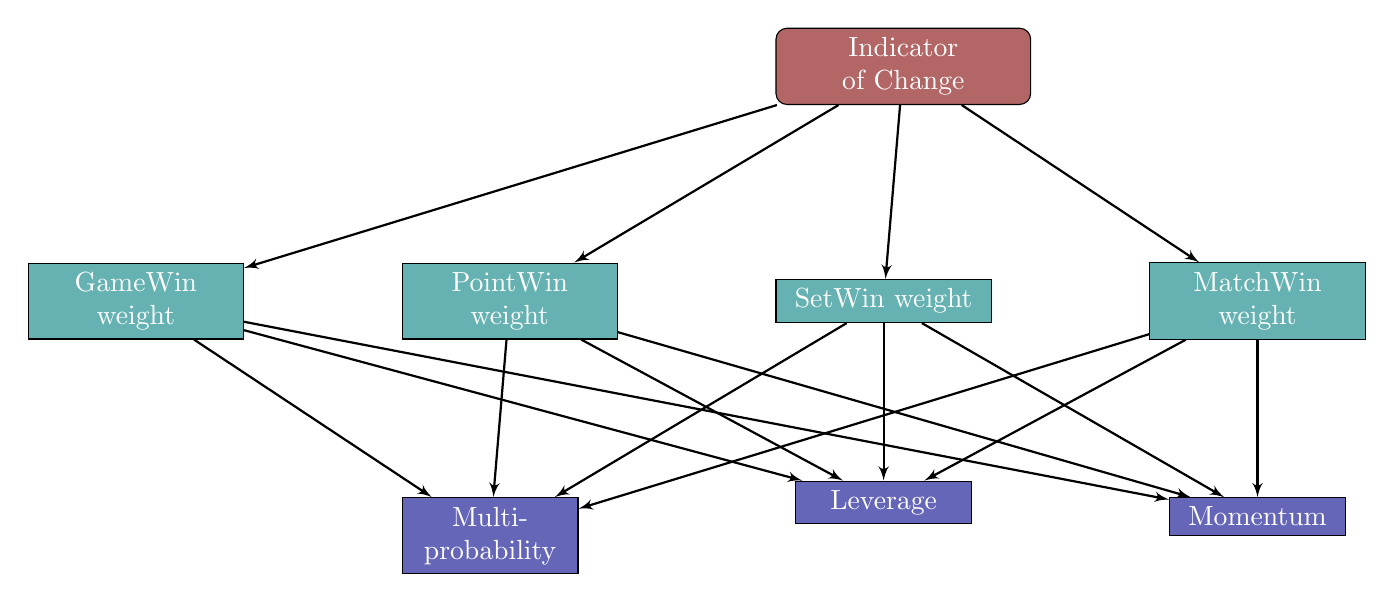
\begin{tikzpicture}[node distance=2cm and 2cm,
    goal/.style={rectangle, rounded corners, draw, fill=Maroon!60, text width=3cm, align=center, text=white},
    criterion/.style={rectangle, draw, fill=Teal!60, text width=2.5cm, align=center, text=white},
    option/.style={rectangle, draw, fill=DarkBlue!60, text width=2cm, align=center, text=white},
    line/.style={draw, thick, -latex'}]
\centering
\node[goal] (goal) {Indicator of Change};
\node[criterion] (c1) [below left=of goal] {PointWin weight};
\node[criterion] (c2) [left=of c1] {GameWin weight};
\node[criterion] (c3) [right=of c1] {SetWin weight};
\node[criterion] (c4) [right=of c3] {MatchWin weight};

\node[option] (p1) [below right=of c2] {Multi-probability}; 
\node[option] (p2) [below=of c3] {Leverage}; 
\node[option] (p3) [below=of c4] {Momentum}; 

% Connect nodes with lines
\foreach \x in {1,...,4}
  \draw[line] (goal) -- (c\x);
  
\foreach \x in {1,...,3}
  \foreach \y in {1,...,4}
    \draw[line] (c\y) -- (p\x);

\end{tikzpicture}
}
\caption{Relation Map for AHP}
\label{fig:my_map}
\end{figure}

\subsubsection{Influence Factors of Swing}
Various factors influence match flow. We utilize the feature importance of gain and split to assess the significance of features from different perspectives. Fig. \ref{fig:gain} represents the feature importance of gain, while Fig. \ref{fig:split} represents the feature importance of split. The figures indicate that match advantage and running distance are the most crucial factors. When a player takes the lead in the game, the match flow tends to favor them. However, if the player has covered a considerable distance during the match, they may experience fatigue and frustration, leading to a shift in the match flow favoring the opponent.\AIcite{AI3}

Moreover, the excellent performance at every point is also significant, including high ball speed and successful serving. When a player hits runs of high-quality balls, they can seize control of the match flow. Additional factors such as server, breakpoints, unforced errors, and winners also contribute to the fluctuations in match flow.         

\begin{figure}[ht]
    \centering
    \begin{minipage}{0.5\textwidth}
        \centering
        \includegraphics[width=\textwidth]{figures/Feature_importance_gain(Match).png} % first image
        \caption{Feature Importance of gain}
        \label{fig:gain}
    \end{minipage}\hfill
    \begin{minipage}{0.5\textwidth}
        \centering
        \includegraphics[width=\textwidth]{figures/Feature_importance_split(Match).png} % second image
        \caption{Feature Importance of split}
        \label{fig:split}
    \end{minipage}
\end{figure}

\subsection{Strategic Advice Based on the Model}
\subsubsection{Mean and Variance of Momentum}
Based on the momentum calculation we perform, we can conclude certain strategies. The mean and variance of a player's momentum can be used to make judgments. For example, Carlos Alcaraz has a momentum mean of 0.158 and a variance of 0.0679 in match \#1701. The mean can indicate how well he performs in matches, while the variance can indicate the degree to which his momentum is affected by the score of the game. The bigger the mean, the h higher the player's capability; the lower the variance, the higher the stability of the player's mindset.

\subsubsection{Factors from the Raw Data}
\begin{figure}[ht]
    \centering
    \begin{minipage}{0.32\textwidth}  % Adjust the width based on your preference
        \centering
        \includegraphics[width=\textwidth]{figures/network1.png}
        \caption{Match network}
        \label{fig:Match network}
    \end{minipage}\hfill
    \begin{minipage}{0.32\textwidth}
        \centering
        \includegraphics[width=\textwidth]{figures/network2.png}
        \caption{Relation network}
        \label{fig:Relation network}
    \end{minipage}\hfill
    \begin{minipage}{0.32\textwidth}
        \centering
        \includegraphics[width=\textwidth]{figures/clustering.png}
        \caption{Players clustering}
        \label{fig:Players clustering}
    \end{minipage}
\end{figure}
Factors like running distances and technical abilities, especially serving proficiency, determine the match outcome. The figures offer strategic advice for pre-match preparation. The figures presented below show different scenarios in a match. In Fig. \ref{fig:Match network}, individuals higher up on the tree have participated in more matches, indicating their increasing match experience. In Fig. \ref{fig:Relation network}, the people in the center with more arrows outward have won more matches, reflecting their relative strength. Fig. \ref{fig:Players clustering} shows the clustering of players based on the relationship between average scores and average running distances.

Our advice is as follows: Pay attention to experienced opponents positioned higher on the tree trunk in Fig. \ref{fig:Match network} and Fig. \ref{fig:Relation network}. Observe your tactics and personal strengths. In Fig. \ref{fig:Players clustering}, Players on the main diagonal tend to have higher scores due to the effort they put into matches. Those in the upper left quadrant achieve more with less effort. On the lower right quadrant, players are good at accurately assessing the situation. Look for opportunities to exploit weaknesses and develop targeted strategies for success.

\section{TASK IV: Test and Generalization}
\subsection{Task Review}
In this task, our objective is to evaluate the generalization capability of our model by applying it to diverse tennis and sports competitions. To achieve this, we obtain the data pertaining to the 2023 US Open competition from online sources and subsequently employ our model to predict match outcomes. Furthermore, we opt to extend our evaluations to badminton, facilitating a comparative analysis between the two sports to discern potential nuances.

In adapting our model to the US Open data, data cleaning is performed, and relevant features are extracted to align with our model's input requirements. For further assessments, we visually analyze the badminton data, exploring the potential application of our model to badminton and its transferability to other sports. This systematic approach ensures the adaptability and effectiveness of our model across diverse sports domains.

\subsection{Test on other Tennis Competition}
Various tennis tournaments are held on different surfaces of the court, each influencing the strategies and techniques of the players, resulting in different performance outcomes. For instance, Wimbledon unfolds on grass courts, while the US Open takes place on hard courts. \AIcite{AI4}The adaptation to these distinct court types requires customized approaches by players. In addition, gender differences introduce an additional layer of sensitivity to court-specific features.

To comprehensively assess diverse tennis competitions, including disparities in competition level, court types, and gender dynamics, we choose to analyze the US Open data from 2023. This dataset comprises over 40,000 rows of information, including both male and female participants. The dataset is carefully curated to align with the characteristics of the given data. After data cleaning procedures, the refined dataset is subjected to our trained model, and its predictive accuracy is evaluated.

The results of this analysis reveal an accuracy rate that exceeds 70\% Table\ref{tab:usopen_report}, indicating its utility in calculating player momentum during matches. This outcome signifies the model's commendable ability to generalize across various tennis competitions. Such empirical evidence also highlights the model's effectiveness in navigating factors like competition level, court type, and gender dynamics within the domain of tennis data analysis.

\begin{table}[ht]
\centering
\caption{Classification Report of US open data}
\label{tab:usopen_report}
\begin{tabular}{lcccc}
\toprule
Class & Precision & Recall & F1-score & Support \\
\midrule
0 & 0.79 & 0.64 & 0.71 & 22616 \\
1 & 0.65 & 0.80 & 0.72 & 19264 \\
\midrule
\textbf{Accuracy} & & & \textbf{0.71} & \textbf{1307} \\
\textbf{Macro Avg} & \textbf{0.72} & \textbf{0.72} & \textbf{0.71} & \textbf{41880} \\
\textbf{Weighted Avg} & \textbf{0.73} & \textbf{0.71} & \textbf{0.71} & \textbf{41880} \\
\bottomrule
\end{tabular}
\end{table}


\subsection{Practicability on other Sports}
We analyze badminton competition data obtained from online sources. Similar to tennis, various features in badminton, such as nations, genders, and levels of matches, exert discernible influences on match results, as illustrated in the following figures.
Despite these similarities, badminton differs from tennis in rule structure, necessitating adjustments to the model's feature inputs. To quantify player momentum in badminton competitions, we devise a strategy. Initially, we extracted key features like match points, nationalities, genders, and match levels. Additionally, these extracted features are used as input to the model, generating predictions across the four possible outcomes. Finally, employing established mathematical formulas, we compute player momentum while carefully considering the unique characteristics of badminton competitions.

\begin{figure}[ht]
    \centering
    \begin{minipage}{0.35\textwidth}
        \centering
        \includegraphics[width=\textwidth]{figures/badminton/All_match_eval_per_tournament_proportion.png} % first image
        \caption{All match eval per tournament proportion}
        \label{fig:All match eval per tournament proportion}
    \end{minipage}
    \begin{minipage}{0.35\textwidth}
        \centering
        \includegraphics[width=\textwidth]{figures/badminton/All_match_eval_per_discipline_proportion.png} % second image
        \caption{All match eval per discipline proportion}
        \label{fig:All match eval per discipline proportion}
    \end{minipage}
    \begin{minipage}{0.3\textwidth}
        \centering
        \includegraphics[width=\textwidth]{figures/badminton/All_match_eval_proportion.png} % second image
        \caption{All match eval proportion}
        \label{fig:All match eval proportion}
    \end{minipage}
    \begin{minipage}{0.35\textwidth}
        \centering
        \includegraphics[width=\textwidth]{figures/badminton/Net_win_change.png} % second image
        \caption{Net win change}
        \label{fig:Net win}
    \end{minipage}\hfill
\end{figure}

\subsection{Possible Improvements}
\subsubsection{Data Segmentation}
In previous work in section \ref{ahp}, the weights derived from AHP remain constant, with the smallest weight assigned to the win probability of a point. However, in actual tennis matches, critical moments such as break points and tie points significantly influence the current match dynamics. To enhance the model's responsiveness, we incorporate these factors into our segmentation strategy. Specifically, at break points and tie points, we amplify the weight assigned to the win probability of a win, highlighting the crucial nature of these pivotal moments.

Following the segmentation adjustments, our model exhibits heightened sensitivity to changes in time and demonstrates improved performance in predicting momentum shifts.

\subsubsection{Additional Feature}
While the model has demonstrated performance and generalization ability, further enhancement is possible through the inclusion of additional insightful features. After acquiring data from various tennis competitions, we proceed to visualize the winner's shot placement in a single match Fig. \ref{figure:tennis shot}. This visual representation suggests potential correlations between shot placement and win probability. Similarly, the spatial position of the winner may also exhibit relative patterns.

However, most competitions lack this detailed information, and therefore, the potential for improvement depends on the enhancement of data collection practices.

\begin{figure}[ht]
    \centering
    \begin{minipage}{0.6\textwidth}
        \centering
        \includegraphics[width=\textwidth]{figures/tennis.png} 
        \caption{The tennis placement of winner}
        \label{figure:tennis shot}
    \end{minipage}\hfill
\end{figure}

\section{Conclusions}
In this study, we introduce three pivotal concepts: multi-probability, leverage, and momentum, and explore their roles in understanding tennis dynamics. Additionally, We design a Multi-LGBM model to predict player performance and analyze match dynamics.

Based on the counter-factual analysis, this Multi-LGBM model integrates the AHP and multi-probability calculations to determine leverage. By applying the EWMA to this leverage, we successfully derive the concept of momentum, which is the focal point of our research. Our novel application of the Multi-LGBM chain offers deeper insights into the intricacies of match dynamics and player strategies.

Our experimental analysis indicates that the Multi-LGBM model is a robust tool for predicting performance in tennis matches. We find that the calculated momentum is a crucial factor in match outcomes. Additionally, we observed that match flow, quantified by multi-probability, is closely related to players' running distance during the match and the quality of their hits.

Further testing on diverse datasets has affirmed the model's robustness and reliability in various scenarios. We've also enhanced the model's accuracy through data segmentation, thereby improving its predictive capabilities.

Drawing on these insights, we offer practical advice to coaches and players. Our recommendations are designed to deepen their understanding of tennis dynamics, thereby enabling them to refine their strategies and performance during matches. These strategies, rooted in a data-driven understanding of tennis, are aimed at helping players and coaches achieve better outcomes in matches.



\begin{thebibliography}{99}
\bibitem{1}Seidl, Robert \& Lucey, Patrick. (2022). Live Counter-Factual Analysis in Women's Tennis using Automatic Key-Moment Detection. %核心论文,关于模型构建的
\bibitem{2} \url{https://theanalyst.com/na/2022/03/capturing-momentum-in-tennis/}%网址
\bibitem{3} Noel, J.T.P. \& Prado da Fonseca, V. \& Soares, A. A Comprehensive Data Pipeline for Comparing the Effects of Momentum on Sports Leagues. Data 2024, 9, 29. https://doi.org/10.3390/data9020029%关于momentum的
\bibitem{4} De Seranno, A., De Pessemier, T., \& Martens, L. (2020). Predicting Tennis Matches Using Machine Learning.

\bibitem{5} \url{https://nycdatascience.com/blog/student-works/data-analysis-on-tennis-player-performance/}
\bibitem{6} Yue JC, Chou EP, Hsieh MH, Hsiao L-C (2022) A study of forecasting tennis matches via the Glicko model. PLoS ONE 17(4): e0266838. https://doi.org/10.1371/journal.pone.0266838
\bibitem{7} S. Jhawar, "Predicting Tennis Match Outcomes," 2022 International Conference on Futuristic Technologies (INCOFT), Belgaum, India, 2022, pp. 1-4, doi: 10.1109/INCOFT55651.2022.10094479.
\bibitem{8} Allen, N. D., Templon, J. R., McNally, P. S., Birnbaum, L., \& Hammond, K. (2010). StatsMonkey: A data-driven sports narrative writer. In Computational Models of Narrative, Papers from the AAAI Fall Symposium, Technical Report (pp. 2-3). (AAAI Fall Symposium Technical Report; Vol. FS-10-04). AI Access Foundation.
\bibitem{9} T. Barnett and S. R. Clarke, "Combining player statistics to predict outcomes of tennis matches," in IMA Journal of Management Mathematics, vol. 16, no. 2, pp. 113-120, Jan. 2005, doi: 10.1093/imam/dpi001.
\bibitem{10} Stephanie Kovalchik, Machar Reid,
A calibration method with dynamic updates for within-match forecasting of wins in tennis, International Journal of Forecasting, Volume 35, Issue 2,2019, Pages 756-766, ISSN 0169-2070,
\bibitem{11} Ke G, Meng Q, FinlT T, et al. Lightgbm: A highly efficient gradient boosting decision tree[C]//Advances in Neural Information Processing Systems. 2017: 3146-3154.
    
\end{thebibliography}
% 
\begin{appendices}
%% Generate the Memorandum if it's needed.
\memoto{Training Coaches of Tennis Players}
\memofrom{MCM Team \#2400430}
\memosubject{Insights into Tennis Momentum: Strategies for Coaches}
\memodate{\today}
% \memologo{}

\begin{memo}[Memorandum]
\newpage
Dear Coach,

I hope this message finds you well. Our team have found that the momentum, which people may regard as randomness, can impact on competition. Our quantified measure of momentum has shown a strong ability to predict the flow of matches, correlating highly with actual outcomes. In our upcoming article, we will present our research on the factors that influence momentum and how players can utilize momentum to their advantage. We believe that our findings will be greatly beneficial in formulating match strategies and training athletes.\AIcite{AI5}

For a start, please allow me to summarize our research findings on momentum. Building on various previous studies, we have developed a complex definition of momentum. We define it as a historical force that is related to the previous state, reflecting the impact of each point on the various levels of winning probabilities in a match. Our model predicts that changes in momentum are closely linked to shifts in the course of the match. During the game, an increase in momentum often leads to consecutive scoring by the player or a significant improvement in their chances of winning the set, playing a crucial role in propelling the player to overcome their opponent.

We have created a heatmap in Fig. \ref{fig:correlation} that shows the correlation between momentum and win probabilities in point, game, set, and match, as well as consecutive scoring by players. These maps clearly indicate that the correlation between momentum and overall match-winning probabilities is significantly stronger compared to smaller units of the game. This suggests that momentum is an indicator that reflects a broader perspective of the game. By analyzing the correlation, we strongly suggest focusing on the momentum flow of a player to represent their match styles. Utilizing the average and variances of momentum, we can judge a player's playing style. For example, if a player's momentum variance is high, it indicates that they are more easily affected by events in the match, suggesting a relatively weak mindset, and vice versa.

Furthermore, the average can demonstrate the player's overall control level. Therefore, you can choose the appropriate opponent and give proper signals during the game based on the player's mindset. For example, suppose your player's momentum is unstable but has a relatively high average; you should encourage them when they are temporarily in an underdog situation, reminding them don't pay much attention to the current losing point and trust in their ability to win back the game, much like Alcaraz's victory over Djokovic in the first match of 7th round in Wimbledon 2023.

As for the on-court situations, we've found that running distance significantly impacts momentum, which tends to decrease when players run long distances continuously. Therefore, it's advisable to manage momentum evenly throughout the match. Players should aim to force their opponents to run more by hitting the ball to distant areas, thereby diminishing their opponent's momentum. Regular training should include a focus on cardiopulmonary fitness, enhancing performance during extended running sequences. Additionally, break points play a crucial role in shifting momentum. Players should be alert to these opportunities, as capitalizing on break points can significantly boost their chances of winning the game.

Sincerely hope that these suggestions can really make a contribution to the players!

Best Regards,

MCM Team \#2400430

\end{memo}

\end{appendices}


\AImatter

\begin{ReportAiUse}{9}

\bibitem{AI1}
OpenAl ChatGPT4 (Feb 2, 2024 version)\\
According to Alcaraz (the server), hit a 130 serve “Body/Wide” of the returner (we saw it was a first serve previously) and close to the li,ne denoting in or out of play. Jarry (the returner) returned the ball 'Deep' on the court (so near the other end of the court) to analyze these words (insert a capture of the CSV file).

Output: This image appears to be a table that lists the abbreviations for width of serve, depth of serve, and depth of return in tennis. Here are possible interpretations of these abbreviations based on tennis terminology:

serve\_width.

BC: Body Center - serves to the middle of the body
B: Body - serve to the body
BW: Body wide - serve to the outside of the body
W: Wide - serve to the sideline of the court
C: Centre - serve at the center of the court
NA: Not applicable - not applicable or no serve data available
serve\_depth.

CTL: Close-to-line - serve close to the baseline
NCTL: Not Close To Line - serve is not close to the baseline
NA: Not Applicable - Not applicable or no serve data available
return\_depth.

ND: Near the baseline, Deep - Ball returned deep near the baseline
D: Deep in the court - The ball went back deep in the court
NA: Not applicable - not applicable or no return data available
These abbreviations are used to record positional information for each serve and return. Based on these abbreviations, a coach or analyst can understand a player's serving strategy and the quality of the Receiver's return. For example, if a player frequently serves 'Wide' and 'Close To Line,' they may be trying to pull their opponent to the edge of the court to gain an advantage in the match. If the return is usually 'Deep,' this may indicate that the Receiver can effectively hit the ball back near the opponent's baseline, which is an excellent defensive strategy.

\bibitem{AI2}
OpenAl ChatGPT4 (Feb 2, 2024 version)\\
Query2: Explain my idea of making a Data Collection based on this Python script (attached data\_process.py)\\
Output: In your data collection process, you have focused on transforming raw tennis match data from a CSV file into a format suitable for analysis. This involves parsing various data types, such as converting time strings to seconds and mapping tennis scores to their numerical unique values like 'Love' or 'Advantage.' The functions are tailored to handle the unique aspects of tennis data, such as interpreting shot types and serving dimensions. Special attention is given to anomalies like 'NA' values, ensuring they are appropriately managed. The script systematically processes each data point, normalizing and standardizing it to make it uniform and interpretable for subsequent analysis. This approach ensures the dataset is accurately represented and ready for detailed analytical tasks.

\bibitem{AI3}
OpenAl ChatGPT4 (Feb 2, 2024 version)\\
Query3: Help me write a latex code to display two images side by side\\
Output: To display two images side by side in LaTeX, you can use the minipage environment in conjunction with the Graphicx package for handling images. Below is a sample LaTeX code snippet for displaying two images side by side:
\lstinputlisting[language=TeX]{code/test.tex}

\bibitem{AI4}
OpenAl ChatGPT3.5 (Feb 5, 2024 version)\\
Query4: What are the four Grand Slam tennis tournaments, and what are their court surfaces?\\
Output: The four Grand Slam tennis tournaments are:
Australian Open - Hardcourt
French Open (Roland Garros) - Clay court
Wimbledon - Grass court
US Open - Hardcourt



\bibitem{AI5}
OpenAl ChatGPT4.0 (Feb 6, 2024 version)\\
Query5: How to write a memo?\\
Output: Title: Usually "Memo".
To: Specify the main recipient of the memo.
From: Write down your name and position.
Date: The date when the memo is written.
Subject: Concisely and clearly describe the main content of the memo.
Body:
Introduction: Briefly introduce the purpose and background of the memo.
Detailed Content: Clearly and specifically state the information you wish to convey. Use paragraphs, lists, or subheadings to organize the information for clarity.
Conclusion or Call to Action: If applicable, summarize the main points and propose the next steps or suggestions.
Attachments: Mention here if there are any accompanying documents.

\end{ReportAiUse}

\end{document}